\documentclass[10pt,nofootinbib]{revtex4}
%\usepackage{ctex}
\usepackage{amsmath,amssymb,amsfonts,mathrsfs,bm,dsfont}
\usepackage{graphics,color}
%\usepackage{hyperref}
\usepackage{tikz}
\usetikzlibrary{arrows}

\newcommand*\dd{\mathop{}\!\mathrm{d}}
\newcounter{Claim}[section]
\newenvironment{Claim}[1][]{{\par\normalfont\bfseries \underline{Claim~\stepcounter{Claim}\arabic{Claim}.}~#1~~}}{\par}
\newcounter{Proposition}[section]
\newenvironment{Proposition}[1][]{{\par\normalfont\bfseries \underline{Proposition~\stepcounter{Proposition}\arabic{Proposition}.}~#1~~}}{\par}
\newcounter{Note}[section]
\newenvironment{Note}[1][]{{\par\normalfont\bfseries \underline{Note~\stepcounter{Note}\arabic{Note}.}~#1~~}}{\par}
\newcounter{Lemma}[section]
\newenvironment{Lemma}[1][]{{\par\normalfont\bfseries \underline{Lemma~\stepcounter{Lemma}\arabic{Lemma}.}~#1~~}}{\par}
\newcounter{Corollary}[section]
\newenvironment{Corollary}[1][]{{\par\normalfont\bfseries \underline{Corollary~\stepcounter{Corollary}\arabic{Corollary}.}~#1~~}}{\par}
\newenvironment{Proof}{{\par~{\normalfont\bfseries $\vartriangleright$}~~}}{\hfill $\square$\par\hfill\par} %\par
\newcounter{Def}[section]
\newenvironment{Def}[1][]{{\par\normalfont\bfseries \underline{Definition~\stepcounter{Def}\arabic{Def}.}~#1~~}}{\par}


\def\Re{\mathop{\mathcal{R}e}}
\def\Im{\mathop{\mathcal{I}m}}
\def\Z{\mathcal{Z}}
\numberwithin{equation}{section}

\begin{document}
\title{Duality in Condensed Matter Physics---From Lattice Models to Bosonic Particle-Vortex Duality}% Force line breaks with \\
%\thanks{This is a reminiscent note for Hubbard-Stratonovich Transformation.}%

\author{Xiaodong Hu}
%\altaffiliation[Also at ]{Boson College}
\email{xiaodong.hu@bc.edu}
\affiliation{Department of Physics, Boston College, MA 02135, USA}

\date{\today}


\begin{abstract}
	In this note, I will review many important dualities in condensed matter physics, from exact dualities on lattice to IR dualities in continuous field theory. As a window to modern study of fermionic particle/vortex duality in FQHE \cite{son2015composite}, deconfined quantum criticality \cite{senthil2004deconfined}, topological insulators \cite{murugan2017particle}, and the brilliant unified work of duality web \cite{seiberg2016duality,senthil2019duality}, old bosonic Particle/Vortex duality is discussed in details. 
\end{abstract}
\maketitle
\tableofcontents
\section{Dualities of Statistical Models}
	\subsection{Quantum-Classical Mapping}
		As a warm-up, let us start with our familiar $d=1$ classical Ising model with \emph{periodic boundary condition}
		\begin{equation}\label{1.1.1}
			-\beta H_{C}=K\sum_{\ell=1}^{N_\tau}s_\ell^zs_{\ell+1}^z+h\sum_{\ell=1}^{N_\tau}s_\ell^z,
		\end{equation}
		where we denote the number of sites as $N_\tau$. Subscript $\tau$ is added for future usage. With the help of well-known \emph{transfer matrix method} we've learned on class, the partition function of \eqref{1.1.1} can be written as 
		\begin{equation}\label{1.1.2}
			\Z=\mathrm{Tr}\bigg((T_1 T_2)^{N_\tau}\bigg),
		\end{equation}
		with
		\begin{equation*}
			T_1\equiv \left(\begin{array}{cc}
				e^K & e^{-K} \\ e^{-K} & e^K
			\end{array}\right),\quad
			T_2\equiv \left(\begin{array}{cc}
				e^h & \\
				& e^{-h}
			\end{array}\right). 
		\end{equation*}
		\indent Now let us take the \emph{scaling limit} \cite{sachdev2011quantum}, where \textbf{we regrad the $d=1$ configuration of lattice (a line) as a new kind of discrete time\footnote{Note that in statistical model (in equilibrium), there is no concept of time.} and identify such line with the path of evolution of one \emph{quantum spin}, namely, the worldline in $(0+1)$-D spacetime}. Under such continuum limit, the space of lattice $a$ goes to zero and the number of sites $N_\tau$ goes to infinity such that the lattice total length $L_\tau\equiv N_\tau a$ is fixed finite\footnote{One should be clear that this is NOT the same as usual \emph{thermodynamic limit}.} (which, as we will see later, corresponds to the finite inverse temperature of its quantum counterpart). But to complete the definition of scaling limit, we also have to assign the manner of coupling constants $K$ and $h$ under the change of $a$ and $N_\tau$.\par
		In fact, correlation length $\xi$ is the natural choice bridging bewteen scaling limit and $K$. We already obtained it in class\footnote{Although \eqref{1.1.3} is obtained in \emph{thermodynamic limit}, with $N_\tau\rightarrow\infty$ the larger eigenvalue of $T_1$ still dominates so the two limits coincide with each other.} that
		\begin{equation}\label{1.1.3}
			\dfrac{a}{\xi}=\ln\coth K,
		\end{equation}
		so with $a/\xi\rightarrow0$ we immediately have $e^{-2K}\sim\frac{a}{2\xi}\rightarrow0.$\par
		For $h$, however, there is in general no prior way to define it. But physically when we increase the nearest neighbor interaction, the average external magnetic field experienced per unit length should also go up. The correct answer is $\widetilde{H}\equiv H/a$, but we can leave this relation as a final correspondence.\par
		Now we are ready to perform the quantum-classical mapping. Writting the two-by-two transfer matrix $T_1$ and $T_2$ in terms of Pauli matrices
		\begin{align}
			T_1&\equiv e^K(1+e^{-2K}\sigma^x)\sim e^K e^{a/(2\xi)\sigma^x},\quad T_2\equiv e^{h\sigma_z}\equiv e^{a\widetilde{h}\sigma^z}
		\end{align}
		and using the fact that $e^{aA}e^{aB}=e^{a(A+B)}(1+\mathcal{O}(a^2))$, \eqref{1.1.2} becomes
		\begin{equation*}
			\Z\rightarrow\mathrm{Tr}\bigg((e^Ke^{a(1/(2\xi)\sigma^x+\widetilde{h}\sigma^z )})^{N_\tau}\bigg)=\Z_0\mathrm{Tr}(e^{-L_\tau H_Q})\equiv\Z_0\mathrm{Tr}(e^{-\beta_Q H_Q}),
		\end{equation*}
		under scaling limit, where the irrelevant $\displaystyle\Z_0\equiv\lim_{N_\tau\rightarrow\infty}e^{KN_\tau}$ (though divergence) is pulled out, and by identifying the imaginary time, or inverse temperature $\beta_Q\equiv 1/L_\tau$,
		\begin{equation}\label{1.1.5}
			H_Q\equiv-\dfrac{1}{2\xi}\sigma_x- \widetilde{h}\sigma_z 
		\end{equation}
		is nothing but the corresponding Hamiltonian of $(0+1)$-D \emph{quantum} Ising model (or transverse field Ising model).\par
		The above quantum-classical mapping can be easily generalize to higher dimensions and even almost all the other statistical models. For the latter, like the correspondence between $O(2)$ quantum rotor model and classical XY Chain, $O(3)$ quantum rotor model and classical Heisenberg model, and so on, can be seen in chapter six \cite{sachdev2011quantum}.\par
		Let me go further to discuss the correspondence between $d=2$ classical Ising model with $(1+1)$-D quantum Ising model. The original work is done by analysis of multi-flipping processes \cite{fradkin1978order,kogut1979introduction} or utilizing Trotter formula \cite{suzuki1976relationship}, but to explicitly show the equivalence of both sides, here I will try to illustrate in a reverse direction, starting with quantum Ising model instead
		\begin{equation}\label{1.1.6}
			H_Q=-J \left(\sum_{i}^{N_x}\sigma^z_i\sigma^z_{i+1}+g\sum_i^{N_x}\sigma_i^x\right).
		\end{equation}
		Discretizing the inverse-temperature (imaginary time) axis (where PBC is applied) and introducing again the finite lattice constant $a$ and finite number of sites $N_\tau$, i.e., reversing the scaling limit, we have
		\begin{equation*}
			\Z\equiv\mathrm{Tr} e^{-\beta H_Q}\rightarrow\mathrm{Tr}\bigg((e^{-aH_Q})^{N_\tau}\bigg).
		\end{equation*}
		The same trick can be applied here so that $e^{-aH_Q}=T_1T_2+\mathcal{O}(a^2)$ with
		\begin{equation}\label{1.1.7}
			T_1\equiv\exp \left(aJg\sum_{i}^{N_x}\sigma_i^x\right),\quad T_2\equiv\exp \left(aJ\sum_{i}^{N_x}\sigma_i^z\sigma_{i+1}^z\right).
		\end{equation}
		\indent To recover the Ising Hamiltonian, the left work is to insert a complete set of basis (here is $\sigma_i^z$ eigenstates) for each pair of $T_1T_2$. Denoting the $N_x$ configuration of states as $|\{s_i\}\rangle$ with $s_i=\pm1$, and labeling further the time direction sites as $|s_i(\ell)\rangle$ with $s_i(\ell)=\pm1$, then the partition function becomes
		\begin{equation*}
			\Z\rightarrow\mathrm{Tr}\left(\prod_\ell^{N_\tau}\langle\{s_i(\ell\}|T_1T_2|\{s_i(\ell)\}\rangle\right)=\mathrm{Tr}\left(\prod_\ell^{N_\tau}\prod_i^{N_x}\exp\bigg(aJ s_{i}(\ell)s_{i+1}(\ell)\bigg)\langle\{s_i(\ell)\}|\exp(aJg\sigma_i^x)|\{s_i(\ell)\}\rangle\right).
		\end{equation*}
		\textbf{It's now natural to regard the two-by-two matrix element $\langle\{s_i(\ell)\}|\exp(aJg\sigma_i^x)|\{s_i(\ell)\}\rangle$ on site $i$ as the transfer matrix of nearest-neighbor interactions along the time direction}. Namely, ansazing
		\begin{equation}\label{1.1.8}
			\langle\{s_i(\ell)\}|\exp(aJg\sigma_i^x)|\{s_i(\ell)\}\rangle\equiv A \exp\bigg(Bs_i(\ell)s_i(\ell+1)\bigg),
		\end{equation}
		where
		\begin{equation*}
			A\equiv\dfrac{1}{2}\cosh(2aJg),\quad e^{-2B}\equiv\tanh(aJg).
		\end{equation*}
		Collecting all terms above, we come to the familiar $d=2$ anisotropic classical Ising model
		\begin{equation}\label{1.1.9}
			\Z\rightarrow\Z_0\mathrm{Tr}\,e^{-\beta H_C}\equiv\Z_0\mathrm{Tr}\left\{\exp\left(\sum_{i,\ell}Jas_i(\ell)s_{i+1}(\ell)+Bs_i(\ell)s_i(\ell+1)\right)\right\}.
		\end{equation}
		The anisotropy of spatial and temperal coupling constant is not strange here because in principal there is no equivalence in the origianl spacetime of quantum Ising model.\par
		To sum up this section, let me summarize the dictionary of quantum-classical mapping as following:
		\begin{table}[htp]
			\begin{tabular}{p{8cm}p{6cm}}
				Classical Statistical Models & Quantum Field Theory\\ 
				\hline\hline
				Total Length along ``Time'' Direction & Inverse Temperture \\ 
				Reciprocal of the Correlation Length & (Mass) Gap of Excitations \\ 
			\end{tabular}
			\caption{Quantum-Classical Mapping}
			\label{tab:1}
		\end{table}

	\subsection{Kramers-Wannier Duality}
		The above mapping we reviewed, is formal so physical uninteresting (compared with the main contents we focus on in this review). That is the reason why we call it mapping rather than duality. Now let us come to the first suprisingly \emph{exact} and non-trivial \emph{self-duality} of $d=2$ classical Ising model. It was first observed early to 1940s in \cite{kramers1941statistics} and was found to be able to applied to any Abelian theory in any dimensions \cite{savit1980duality}. Since $d=2$ classical Ising model is equivalent to $(1+1)$-D quantum Ising model, I try to recover the celebrated result in the latter case.\par
		Given a $1$-D chain with Hamiltonian \eqref{1.1.6}, let us define a thoery on its \emph{dual lattice}, i.e., on the link with a new group of operators $\{\mu_i^x,\mu_i^z\}$ such that
		\begin{equation}\label{1.2.1}
			\mu^x_i\equiv\sigma^z_i\sigma_{i+1}^z,\quad \mu^z_i\equiv\sum_{\ell<i}\sigma^x_\ell.
		\end{equation}
		Clearly $\mu_i^x$ and $\mu_i^z$ satisfy the familiar algebra of Pauli matrix that
		\begin{equation*}
			(\mu_i^z)^2=(\mu_i^x)^2=1,\quad \{\mu_i^x,\mu_i^z\}=0.
		\end{equation*}
		So $\sigma_i^x\equiv \mu_i^z\mu_{i+1}^z$ and the original Hamiltonian can be expressed in terms of operators on the link
		\begin{equation}\label{1.2.3}
			H_Q=-J \left(\sum_i\mu_i^x+g\sum_i\mu_i^z\mu_{i+1}^z\right).
		\end{equation}
		Hamiltonian \eqref{1.2.3} and \eqref{1.1.6} take exactly the same form, except for the difference on the position of coupling constants. In fact, by pulling out a common factor $g$, we conclude nonperturbatively on Hamiltonian level that
		\begin{equation}\label{1.2.4}
			H_Q(\sigma;\lambda)\equiv g H_Q(\mu;1/g).
		\end{equation}
		\indent Self-duality \eqref{1.2.4} is a powerful result. \textbf{It is a first non-trivial example of modern concept of \emph{strong-weak duality} \cite{senthil2019duality}: mapping the strong coupling (or high-terperature phase, in its classical counterpart) $g>1$ to the weak coupling $1/g$}. It also implies that each energy eigenvalue satisfies $E(g)\equiv gE(1/g)$, so it provides a nonperturbative check of the excitation spectrum. Furthermore, if we assumes\footnote{Kramers and Wannier assume this fact. Wigner prove it.} the uniqueness of the gap vanishing point, we immediately obtain the critical point of $(1+1)$-D quantum Ising model
		\begin{equation}\label{1.2.5}
			g_c=1,
		\end{equation}
		or eqiuvalent, the critical point of $d=2$ classical Ising model! This is an amazing byproduct because in the past before Onsager\footnote{Historically, Onsager did obtain the exact solution far before the invention of RG. But here I just want to emphasize the power of Kramers-Wannier duality.}, we have no idea where the exact critical point is, but can only perturbatively approach it by RG transformation, as we have done in class. 

	\subsection{$\mathbb{Z}_2$ Gauge Theory}
		The above string operator technique \eqref{1.2.1} can also be applied to higher dimensions and lead us to more novel statistical models. We start with the simplest $\mathbb{Z}_2$ gauge field, which describes the fluctuation of loops on infinitely large square lattice. Spin degree of freedoms are placed on the \emph{links} of sites, with the Hamiltonian
		\begin{equation}\label{1.3.1}
			H_{\mathbb{Z}_2}=-K\sum_\square\prod_{\ell\in\square}\sigma_\ell^z-g\sum_\ell\sigma_\ell^x.
		\end{equation}
		Hamiltonian \eqref{1.3.1} possesses local $\mathbb{Z}_2$ gauge symmetry since it commutes with the operator $\displaystyle G_i\equiv\prod_{\ell\in+}\sigma_\ell^x$ on each site and $G_i^2\equiv1$. Without loss of generality, let us fix the gauge by setting $G_i\equiv1$. Then again by introducing operator on the site of \emph{dual} lattice
		\begin{equation}\label{1.3.2}
			\mu^x_i\equiv\prod_{\ell\in\square_i}\sigma^z_\ell,\quad \mu_i^z\equiv\prod_{\ell\in\mathcal{C}}\sigma_\ell^x,
		\end{equation}
		where set $\mathcal{C}$ is the intersection of right ray with original lattice, as is illustrate in FIG. \ref{fig:1}.
		\begin{figure}[!htp]
			\centering
			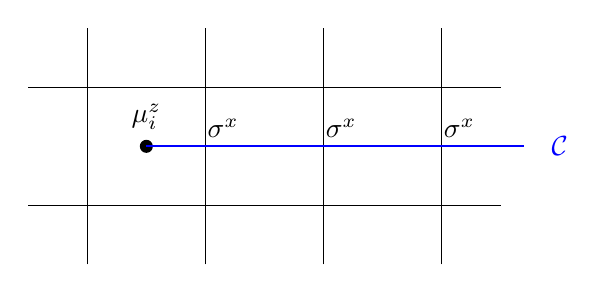
\begin{tikzpicture}[scale=1.5]
				\draw[step=1cm] (0.5,0.5) grid (4.5,2.5);
				\node[circle,fill=black,scale=0.5,label={$\mu_i^z$}] at (1.5,1.5) {};
				\draw[thick,blue] (1.5,1.5) to (4.7,1.5);
				\foreach \x in {1,...,3}{
					\node at (\x+1.15,1.65) {$\sigma^x$};
				}
				\node at (5,1.5) {\color{blue}$\mathcal{C}$};
			\end{tikzpicture}
			\caption{{\bf String Operator}.}
			\label{fig:1}
		\end{figure}
		It is clear that $\mu_i^x$ and $\mu_i^z$ again satisfy the algebra of Pauli matrix
		\begin{equation*}
			(\mu_i^z)^2=(\mu_i^x)^2=1,\quad \{\mu_i^x,\mu_i^z\}=0.
		\end{equation*}
		And noting that $\sigma^x$ on vertical edges and horizental edges can be directly read from FIG. \ref{fig:2}.\par 
		\begin{figure}[!htp]
			\centering
			\begin{minipage}{.4\textwidth}
				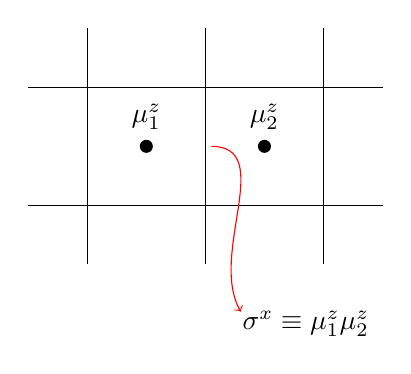
\begin{tikzpicture}[scale=1.5]
					\draw[step=1cm] (0.5,0.5) grid (3.5,2.5);
					\node[circle,fill=black,scale=0.5,label={$\mu_1^z$}] at (1.5,1.5) {};
					\node[circle,fill=black,scale=0.5,label={$\mu_2^z$}] at (2.5,1.5) {};
					\draw [->,red] (2.05,1.5) to [out=0,in=120] (2.3,0.1);
					\node at (2.85,0) {$\sigma^x\equiv \mu_1^z\mu_2^z$};
				\end{tikzpicture}
			\end{minipage}
			%\hspace{0.2\textwidth}
			\begin{minipage}{.5\textwidth}
				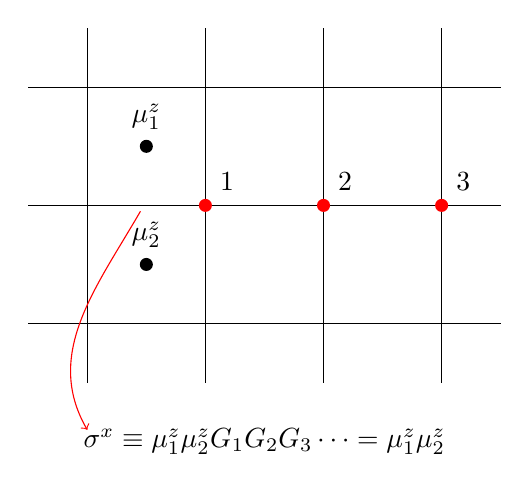
\begin{tikzpicture}[scale=1.5]
					\draw[step=1cm] (0.5,0.5) grid (4.5,3.5);
					\node[circle,fill=black,scale=0.5,label={$\mu_2^z$}] at (1.5,1.5) {};
					\node[circle,fill=black,scale=0.5,label={$\mu_1^z$}] at (1.5,2.5) {};
					\foreach \x in {1,...,3}{
						\node[circle,fill=red,scale=0.5,label={45:\x}] at (\x+1,2) {};
					}
					\draw [->,red] (1.45,1.95) to [out=240,in=120] (1,0.1);
					\node at (2.5,0) {$\sigma^x\equiv \mu_1^z\mu_2^zG_1G_2G_3\cdots=\mu^z_1\mu^z_2$};
				\end{tikzpicture}				
			\end{minipage}
			\caption{$\sigma^x$ on vertical and horizental links.}
			\label{fig:2}
		\end{figure}
		So finally we come to the $(2+1)$-D quantum Ising model
		\begin{equation}\label{1.3.3}
			H=-g\sum_{\langle ij\rangle }\mu_i^z\mu_i^z-K\sum_i\mu_i^x,
		\end{equation}
		with the exchange of coupling constants $K$, as expected.

\section{IR Dualities of Continuous Field Theory}
		So far we are just playing with simple lattice models. In this section, we try to give some specific physical realizations, their \emph{low-energy effective} theories and to reveal their dualities.\par
	\subsection{Superfluid-Insulator Transition and Bose-Hubbard Model}
		Enlighted by the well-know weak interacting bosonic theory for superfluidity and the picture of Cooper pairs, Fisher \textit{et al.} first propose the celebrated soft-core \emph{Bose-Hubbard model} in studying of superfluid-Mott Insulator phase transion \cite{fisher1989boson}
		\begin{equation}\label{2.1.1}
			H=-w\sum_{\langle ij\rangle }(b_i^\dagger b_j+b_j^\dagger b_i)-\mu\sum_{i}n_i+\dfrac{U}{2}\sum_{i}n_i(n_i-1),
		\end{equation}
		where $b_i$ and $b_i^\dagger$ are annihilation and creatio operator for Cooper pairs, $w$ is the Josephson tunneling potential of Cooper pairs and $U$ is the on-site repulsion of them. Unlike the usual treatment of the quartic term in \eqref{2.1.1} (for example, in weakly-interacting fermi liquid), here \textbf{we have to start with large-U Mott Insulation region, otherwise in weak coupling limit we will encounter with trivial phase transition between superfluid and normal liquid}. Therefore, we introduce a complex scalar field $\Phi$ and perform the standard Hubbard-Stratonovich transformation to decoupling the hopping term instead. Namely, writting
		\begin{equation*}
			\exp\left(\int\dd\tau\,w\sum_{\langle ij\rangle}n_in_i\right)\equiv\int\mathcal{D}(\bar{\Psi},\Psi)\,\exp\left[-\int\dd\tau\left(\sum_{i,j}\bar{\Psi}w_{i,j}^{-1}\Psi-\sum_{i}(\bar{b}_i\Psi_i+\bar{\Psi}_ib_i)\right)\right],
		\end{equation*}
		where $w_{i,j}\equiv w\delta_{ij}$, we have
		\begin{equation*}
			S=\int\dd\tau\left[\sum_i \left(\bar{\Psi}_i(\partial_\tau-\mu)\Psi_i+\dfrac{U}{2}\bar{\Psi}_i\bar{\Psi}_i\Psi_i\Psi_i\right)+\sum_{i,j}\bar{\Psi}w_{i,j}^{-1}\Psi+\sum_{i}(\bar{b}_i\Psi_i+\bar{\Psi}_ib_i)\right].
		\end{equation*}
		Low-energy Effective Hamiltonian is obtained by integrating out $\Psi_i$ fields. But it seems to be impossible at the first glance, for the existence of quartic term above. However, if we can write
		\begin{equation}\label{2.1.2}
			e^{-S_{\text{eff}}}=\Z_{\text{loc}}\,e^{-\int\dd\tau\,\sum_{i,j}\bar{\Psi}_iw_{i,j}^{-1}\Psi_j}\left\langle e^{-\int\dd\tau\,\sum_i(\bar{\Psi}b_i+\bar{b}_i\Psi)}\right\rangle_{\text{loc}},
		\end{equation}
		where
		\begin{equation*}
			\langle A(\bar{b},b)\rangle_{\text{loc}}\equiv\dfrac{1}{\Z_\text{loc}}\int\mathcal{D}(\bar{b},b)\, Ae^{-S_{\text{loc}}},
		\end{equation*}
		and
		\begin{equation}\label{2.1.3}
			S_{\text{loc}}\equiv\int\dd\tau\left[\sum_i \left(\bar{\Psi}_i(\partial_\tau-\mu)\Psi_i+\dfrac{U}{2}\bar{\Psi}_i\bar{\Psi}_i\Psi_i\Psi_i\right)\right],
		\end{equation}
		then because we are interested in large-U limit, the fluctuation field $\Psi$ around critical point can be safely assumed to be small enough so that perturbation theory can be used here. More precisely, we can evaluate the average on extreme Mott regime through \emph{cumulant expansion} $\langle e^{-O}\rangle\sim e^{-\langle O\rangle-(\langle O^2\rangle-\langle O\rangle^2)/2}$ up to the second order. Clearly all terms containing $\langle\Psi_i\rangle_{\text{loc}}$ vanishes, so we are left with merely
		\begin{align}
			\dfrac{1}{2}\left\langle\left(\int\dd\tau\,\sum_i(\bar{\Psi}_ib_i+\bar{b}_i\Psi_i)\right)^2\right\rangle_{\text{loc}}&=\dfrac{1}{2}\int\dd\tau\dd\tau'\sum_{i,j}\bigg\langle\bar{\Psi}_i(\tau)\Psi_j(\tau')b_i(\tau)\bar{b}_j(\tau')+h.c.\bigg\rangle_{\text{loc}}\nonumber\\
			&=\int\dd\tau\dd\tau'\sum_{i}\bar{\Psi}_i(\tau)\Psi_j(\tau')\langle T_\tau\{b_i(\tau)\bar{b}_j(\tau')\}\rangle_{\text{loc}}\nonumber\\
			&\equiv-\int\dd\tau\dd\tau'\sum_i\bar{\Psi}_i(\tau)G(\tau-\tau')\Psi_i(\tau'),\label{2.1.4}
		\end{align}
		Average in \eqref{2.1.4} is evaluable now because local average is taken on-site (so only $i=j$ terms are left). Green function $G(\tau-\tau')$ can also be obtained if weinput the known energy level in extreme Mott regime ($w=0$) that $\varepsilon_n\equiv Un(n+1)/2-\mu n$ and work in such energy basis
		\begin{equation}\label{2.1.5}
			G(\tau)=-\dfrac{1}{\Z_{\text{loc}}}\sum_{m}\langle m|e^{\tau H}\psi(0)e^{-\tau H}\bar{\psi}(0)e^{-\beta H}|m\rangle=-\dfrac{1}{\Z_{\text{loc}}}\sum_m (m+1)e^{-\beta \varepsilon_m}e^{\tau(\varepsilon_m- \varepsilon_{m-1})},
		\end{equation}
		or in frequency space with the low-temperature limit (we are interested in quantum phase transition) $\beta\rightarrow\infty$ that
		\begin{equation}\label{2.1.6}
			G(i\omega_n)=\dfrac{n+1}{i\omega_n+\varepsilon_n- \varepsilon_{n+1}}+\dfrac{n}{i\omega_n+ \varepsilon_{n+1}-\varepsilon_n}=\dfrac{n+1}{i\omega_n+\mu-nU}+\dfrac{n}{i\omega_n+\mu-U(n-1)},\quad i\omega_n\mapsto\omega+i\delta 
		\end{equation}
		Collecting all terms above, finally we come to the effective action in momentum space 
		\begin{equation}\label{2.1.7}
			S_{\text{eff}}=-\sum_{\bm{q},i\omega_n}\bar{\Psi}_{q}\bigg(-w_{\bm{q}}^{-1}+G(i\omega_n)\bigg)\Psi_q
		\end{equation}
		with $w_{\bm{q}}$ the Fourier transformation of nearest neighbor hopping matrix $w_{\bm{q}}=2w\sum_{\ell=1}^d\cos(q\ell)$.\par
		In the vicinity of quantum phase transition, both $\bm{q}$ and $\omega$ are small, so we can expand the above dressed Green function up to the second order, obtaining
		\begin{equation}\label{2.1.8}
			G_{\text{eff}}^{-1}\simeq G_{\text{eff}}^{-1}(0)+\dfrac{\partial G_{\text{eff}}^{-1}}{\partial i\omega_n}i\omega+\dfrac{\partial^2G_{\text{eff}}^{-1}}{\partial \bm{q}^2}\bm{q}^2+ \dfrac{\partial^2G_{\text{eff}}^{-1}}{\partial (i\omega_n)^2}(i\omega_n)^2.
		\end{equation}
		The above expansion contains only the second derivatives of momentem because $w_{\bm{q}}$ by definition is an even function. Redefining all derivatives above, we come to the \emph{free} low-energy effective Lagragian
		\begin{equation}\label{2.1.9}
			S_{\text{eff}}=\int\dd x\,\left(a\bar{\Psi}\partial_\tau\Psi+|\partial_\tau\Psi|^2+s|\Psi|^2+c^2|\nabla\Psi|^2\right).
		\end{equation}
		Wether we keep the first or the second order time-derivative term in \eqref{2.1.9} depends on the value of $a$, whose explicit form can be read from \eqref{2.1.6} that
		\begin{equation}\label{2.1.10}
			a\equiv\dfrac{\partial}{\partial \mu}\left(\dfrac{n+1}{i\omega_n+\mu-nU}+\dfrac{n}{i\omega_n+\mu-U(n-1)}\right).
		\end{equation}
		\textbf{If $a=0$, there is remarkably an emergent Lorentz symmetry in the low-energy effective theory}. The critical thoery of such model is CFT3, so belongs to the same universal class of $O(2)$ quantum rotor model, or $d=3$ classical XY model \cite{sachdev2011quantum}. If not, the second term should be dropped and we come to a new universal class. Fisher {\it et al.} argued that the vanishing property of $a$ at mean field level continuous to hold when quantum fluctuations are included \cite{fisher1989boson}. So Let us narrow our discussion to the interesting relativistical case in the following literature.\par 
		In order to get an interacting theory, we have to keep more terms in the previous cumulant expansion. But instead, we can accomplish this by simple symmetry argument. Low-energy effective theory here should also keep the original global $U(1)$ symmtry, so the next term must be of quartic order, leaving
		\begin{equation}\label{2.1.11}
			S_{\text{eff}}=\int\dd x\,\left(|\partial_\tau\Psi|^2+c^2|\nabla\Psi|^2+s|\Psi|^2+u|\Psi|^4\right)\equiv\int\dd x\left(|\partial_\mu\Psi|^2+s|\Psi|^2+u|\Psi|^4\right).
		\end{equation}

	\subsection{Bosonic Particle/Vortex Duality}
		\subsubsection{Duality for Classical Vortex}
		Bosonic particle/vortex duality is first proposed by Peskin in study of connection between strongly-coupling $(3+1)$-D Abelian gauge theory and $d=3$ XY model of superconductors \cite{peskin1978mandelstam}, and then numerically verified by Dasgupta and Halperin in study of phase transition of $d=3$ XY model \cite{dasgupta1981phase}. Let me recapitulate their brilliant idea in continuum theory instead. We will start with the \emph{low-energy} effective theory of classical $d=3$ XY model
		\begin{equation}\label{2.2.1}
			\beta H\equiv-\sum_{\langle ij\rangle}J_{ij}\cos(\theta_i-\theta_j)\implies S=\int\dd^3 x\,\dfrac{J}{2}(\partial_\mu\theta)^2,
		\end{equation}
		where we treat one-component of $d=3$ space as Euclidean time so $\partial_\mu\equiv(\partial_\tau,\nabla)$. It is widely known in $d=2$ that instanton effects \cite{nagaosa2013quantum,Wen-QFT} lead to the duality among XY model, Coulomb gas of vortex, and Sine-Gordon model. Similar results occur in $d=3$ (or $2+1$-D here) because $\theta$ is still defined up to $2\pi$ times an integer. Such multi-valued singular behavior may also result in phase transtions. Carefully splitting the normal part and singular part of fields $\theta\equiv\theta_0+\theta_{\mathrm{v}}$, where the vortex configuration centered at $(X_2(\tau),X_1(\tau))$ for each time slice $\tau$ taking the form of
		\begin{equation*}
			\theta_{\mathrm{v}}(\bm{x},\tau)\equiv\arctan\left(\dfrac{x_2-X_2(\tau)}{x_1-X_1(\tau)}\right),
		\end{equation*}
		we can then recognize the \emph{vortex density}
		\begin{equation}\label{2.2.2}
			j_0(x)\equiv\delta(\bm{x}-\bm{X}(\tau))
		\end{equation}
		from $(\partial_\mu \partial_\nu- \partial_\nu \partial_\mu)\theta_{\mathrm{v}}=2\pi\delta(\bm{x}-\bm{X}(\tau))$, and generalize \eqref{2.2.2} to the complete $3$-current
		\begin{equation}\label{2.2.3}
			j_\mu(x)\equiv\dfrac{1}{2\pi}\varepsilon_{\mu\nu\lambda}\partial_\nu \partial_\mu\theta_{\mathrm{v}}(x)
		\end{equation}
		so that the \emph{vortex current density} $\bm{j}(x)=\delta(\bm{x}-\bm{X}(\tau)) \partial_\tau\bm{X}\equiv j_0\bm{v}_{\text{core}}$ as expected.\par
		After all the preliminaries, we can perform Hubbard-Stratonovich transformation with the help of $J_\mu$ (DO NOT mix the auxiliary field $J_\mu$ with vortex current field $j_\mu$)
		\begin{equation}\label{2.2.4}
			\Z=\int\mathcal{D}\theta\mathcal{D}J_\mu\,e^{-S},\quad S=\int\dd x\bigg[\dfrac{1}{2J}J_\mu^2(x)+iJ_\mu(x)(\partial_\mu\theta_0+\partial_\mu\theta_v)\bigg].
		\end{equation}
		After integrating out normal field $\theta_0$, we are left with
		\begin{equation}\label{2.2.5}
			\Z=\int\mathcal{D}\theta_{\mathrm{v}}\mathcal{D}J_\mu\,\exp\left[\dfrac{1}{2J}J_\mu^2+iJ_\mu\partial_\mu\theta_{\mathrm{v}}\right]\prod_{x}\delta(\partial_\mu J_\mu).
		\end{equation}
		Constraint $\partial_\mu J_\mu=0$ can be solved by introducing a vector potential $a_\mu$ such that
		\begin{equation}\label{2.2.6}
			J_\mu\equiv\dfrac{1}{2\pi}\varepsilon_{\mu\nu\lambda}\partial_\nu a_\lambda.
		\end{equation}
		Then interestingly the second interacting term in \eqref{2.2.5} can be related with the vortex current we defined before by dropping a boundary term
		\begin{equation*}
			S_{\text{int}}\equiv i\int\dd x\,J_\mu(x)\partial_\mu\theta_{\mathrm{v}}(x)=i\int\dd x\,\dfrac{1}{2\pi}\varepsilon_{\mu\nu\lambda}\partial_\nu a_\lambda \partial_\mu\theta_{\mathrm{v}}=-i\int\dd x\,a_\lambda\dfrac{1}{2\pi}\varepsilon_{\mu\nu\lambda}\partial_\nu \partial_\mu\theta_{\mathrm{v}}\equiv i\int\dd x\,a_\mu j_\mu.
		\end{equation*}
		Finally, {\bf{we come to the \emph{classical} field theory with the current of vortex playing the role as matter field, interacting through internal $U(1)$ gauge field $a_\mu$}}
		\begin{equation}\label{2.2.7}
			\Z=\int\mathcal{D}a_\mu\mathcal{D}j_\mu\,e^{-S},\quad S=\int\dd x\, \bigg\{ia_\mu(x)j_\mu(x)+\dfrac{1}{8\pi^2 J} (\varepsilon_{\mu\nu\lambda}\partial_\nu a_{\lambda})^2\bigg\}.
		\end{equation}
		{\color{red}Action \eqref{2.2.7} are indeed \emph{first-quantized}} (written in path integral formalism). To put this more clearly, let us introduce the third component of vortex core $X_0\equiv\tau$ and substitute back the explicit form of matter field
		\begin{equation*}
			j_\mu(\bm{x})\equiv \delta(\bm{x}-\bm{X}(\tau))\partial_\tau X_\mu(\tau),
		\end{equation*}
		then
		\begin{equation}\label{2.2.8}
			S=i\int\dd\tau\,a_\mu(x(\tau))\dot{X}_\mu(x(\tau))+\dfrac{1}{8\pi^2 J}\int\dd^3x\,(\varepsilon_{\mu\nu\lambda}\partial_\nu a_{\lambda})^2.
		\end{equation}
		Action \eqref{2.2.7} or \eqref{2.2.8} enlighten us to switch the viewpoint from charged boson to vortex, but clearly $X_\mu$ has no dynamics from \eqref{2.2.8}. \textbf{So we must miss the ``kinetic energy'' of such new vortex-like particles}. We will discuss this below.

		\subsubsection{Quantization of Vortex Loops --- Random Walk}
		There are two obstacles in the way of obtaining the correct duality mapping. On the one hand, \textbf{we are actually considering a \emph{many-body system} of vortex, so naturally the second quantization language should be used}. On the other hand, more seriously, {\bf unlike the usual point-like particle in quantum mechanics, each configuration of vortex, is rather a \emph{closed loop} in $(2+1)$-D spacetime. So besides the action we obtained in \eqref{2.2.8}, we also need to include the self-energy \cite{banks1977phase} of loops themselves}. Physically, such extra term comes from  the UV detail\footnote{Recall that our physical scale is between the sample size IR cutoff and lattice size UV cutoff.} of vortex cores we have missed. Similar to Namb-Goto action in bosonic string theory, the most simplest spacetime translation invaraint action we can write is
		\begin{equation*}
			S_{\text{self}}=A\sum_i\int\dd s_i.
		\end{equation*}
		In combination of many-body interaction with internal gauge field
		\begin{equation*}
			S_{\text{int}}=i\sum_i\int\dd\tau\,a_\mu(\tau) X_{\mu,i}(\tau),			
		\end{equation*}		
		the action waiting for second quantization is
		\begin{equation*}
			S_{\text{vortex}}=S_{\text{self}}+S_{\text{int}}.
		\end{equation*}
		The main problem evaluting $S_{\text{self}}$ is to count the number of configurations. Introducing $P(t)$ the number of possible configuration of \emph{one close loop} consisting $t$ steps, the self-energy part of the action (for one loop) can be alternatively written as
		\begin{equation}\label{2.2.9}
			\Z_{\text{loop}}=\int_0^\infty\dd t\,P(t)e^{-At-S_{\text{int}}}.
		\end{equation} 
		\indent To detemine the form of $P(t)$, let us borrow the idea from \emph{random walk} \cite{stone1978condensed,itzykson1991statistical}, introducing the probability distribution $p(\bm{X'},t;\bm{X},0)$ for the probability of vortex cores reaching the point $\bm{X'}$ from point $\bm{X}$ after $t$ steps. Simple analysis of recurrence relation shows that $p$ obeys diffusion equation \cite{itzykson1991statistical}
		\begin{equation}\label{2.2.10}
			\dfrac{\partial p}{\partial t}=\dfrac{1}{2D}\nabla^2p.
		\end{equation}
		And the total number of paths $\Gamma(\bm{X'},t;\bm{X},0)$ going in $t$ steps from $\bm{X}$ to $\bm{X'}$ is obviously related by (on hypercubic lattice)
		\begin{equation}\label{2.2.11}
			\Gamma(\bm{X'},t;\bm{X},0)\equiv p(\bm{X'},t;\bm{X},0)(2D)^t.
		\end{equation}
		Combination of \eqref{2.2.10} and \eqref{2.2.11} gives
		\begin{equation}\label{2.2.12}
			\dfrac{\partial \Gamma}{\partial t}=\left(\dfrac{1}{2D}\nabla^2+\ln(2D)\right)\Gamma. 
		\end{equation}
		But as is shown below, what we need for single loop partition function is not the single $\Gamma$, but $\Gamma e^{-S_{\text{int}}}$ instead. So let us express $\Gamma$ in path integral formalism. This can be done easily. Noticing that \eqref{2.2.12} takes exactly the same form of Schr\"{o}rdinger equation if we recognizing the differential operator on the RHS of \eqref{2.2.12} as the vortex-like single particle's Hamiltonian, then after Legendre transformation,
		\begin{equation}\label{2.2.13}
			\Gamma(\bm{X'},t;\bm{X},0)\equiv\int_{X(0)=X}^{X(t)=X'}\mathcal{D}X_\mu\,\exp\left(-\int\dd\tau\,\left(\dfrac{D}{2}\dot{X}_\mu^2+\ln(2D)\right)\right),
		\end{equation}
		and
		\begin{equation}\label{2.2.14}
			\widetilde{\Gamma}(\bm{X'},t;\bm{X},0)\equiv\Gamma e^{-S_{\text{int}}}\equiv\int_{X(0)=X}^{X(t)=X'}\mathcal{D}X_\mu\,\exp\left(-\int\dd\tau\,\left(\dfrac{D}{2}\dot{X}_\mu^2+\ln(2D)+ia_\mu\dot{X}_\mu\right)\right),
		\end{equation}
		Boundary condition on the path integral makes the general form of $\Gamma$ hard to find. However, fortunately enough, it is only when $\bm{X'}\equiv\bm{X}$ that $\Gamma(\bm{X},t;\bm{X},0)$ coincides with the total number of configurations for \emph{one close loops} $P$ (up to the $t$ times overcounts of the start point on a loop)
		\begin{equation}\label{2.2.15}
			\int\dd X\,\Gamma(\bm{X},t;\bm{X},0)\equiv tP(t).
		\end{equation}
		On the other hand, we can recover the Schr\"{o}rdinger equation of $\widetilde{\Gamma}$ from \eqref{2.2.14} that
		\begin{equation}\label{2.2.16}
			\dfrac{\partial\widetilde{\Gamma}}{\partial t}=\left(\dfrac{1}{2D}(\partial_\mu+ia_\mu)^2+\ln(2D)\right).
		\end{equation}
		Then $\widetilde{\Gamma}$ can be constructed from its eigenstates
		\begin{equation*}
			\widetilde{\Gamma}(\bm{x'},t;\bm{x},0)\equiv\sum_{n}\psi_n^*(\bm{x'})\psi_n(\bm{x})e^{-E_nt},
		\end{equation*}
		where
		\begin{equation*}
			H_{\widetilde{\Gamma}}\psi_m(\bm{x})\equiv\left(-\dfrac{1}{2D}(\partial_\mu-ia_\mu)^2-\ln(2D)\right)\psi_m(\bm{x})=\widetilde{E}_m\psi_m(\bm{x}).
		\end{equation*}
		

		Colleting all equations above, the single-loop partition function can be evaluated by taking derivatives of $A$ that
		\begin{align*}
			-\dfrac{\partial \ln\Z_{\text{loop}}}{\partial A}&\equiv\int_0^\infty\dd t\, tP(t)e^{-S_{\text{int}}}e^{-At}=\int_0^\infty\dd t\int\dd x\,\bigg(\Gamma(\bm{x},t;\bm{x},t)e^{S_{\text{int}}}\bigg)e^{-At}=\int_0^\infty\dd t\sum_{n}\int\dd x\,\psi_n^*(\bm{x})\psi_n(\bm{x})e^{-(\widetilde{E}_n+A)t}\\
			&=\sum_{n}\int_0^\infty e^{-(\widetilde{E}_n+A)t}=\sum_n\dfrac{1}{\widetilde{E}_n+A}\equiv\mathrm{Tr} \left(-\dfrac{1}{2D}(\partial_\mu-ia_\mu)^2-\ln(2D)+A\right)^{-1},
		\end{align*}
		where in the first line we use the normarlization condition for eigenstates, and in the last line we re-express the summation over all $H_{\widetilde{\Gamma}}$'s eigenvalues as the trace of the differential operator itself. Thus after integrating over $A$,
		\begin{equation}\label{2.2.17}
			\Z_{\text{loop}}=\mathrm{Tr}\ln\left(-\dfrac{1}{2D}(\partial_\mu-ia_\mu)^2-\ln(2D)+A\right)+\text{const}=\ln\det \left(-\dfrac{1}{2D}(\partial_\mu-ia_\mu)^2+m^2\right)+\text{const},
		\end{equation}
		where $m^2\equiv A-\ln(2D)$.\par
		Finally for an ensemble of indistinguishable non-interacting\footnote{As is argued in \cite{banks1977phase}, interaction among vortex loops (of Biot-Savart type) is negligible from their self-energy if the length of loop is large.} loops
		\begin{equation*}
			\Z_{\text{vortex}}=\sum_n\dfrac{(\Z_{\text{loop}})^n}{n!}=e^{\Z_{\text{loop}}}=\text{const}\times{\det}^{-1}\left(-\dfrac{1}{2D}(\partial_\mu+ia_\mu)^2+m^2\right),
		\end{equation*}
		which, can be alternatively written as a function integral over some bosonic quantum field
		\begin{equation}\label{2.2.18}
			\Z_{\text{vortex}}=\int\mathcal{D}\phi\,\exp \left\{-\int\dd x\,\phi^*\left(-\dfrac{1}{2D}(\partial_\mu+ia_\mu)^2+m^2\right)\phi\right\}.
		\end{equation}
		Combining the left part of action of internal gauge field in \eqref{2.2.8}, we finally come to the correct \textbf{dual theory of scalar $\mathrm{QED}_3$}
		\begin{equation}\label{2.2.19}
			S_{\text{dual}}=\int\dd x\, \left\{-\dfrac{1}{2D}|(\partial_\mu-ia_\mu)\phi|^2+m^2|\phi|^2+\dfrac{1}{16\pi^2J^2}f^{\mu\nu}f_{\mu\nu}\right\}.
		\end{equation}
		Interacting $|\phi|^4$ term is missed here because we did not include the repulsion among vortices. You can add it by hand.\par
		To summary up, we have the dictionary for bosonic particle/vortex duality in TABLE \ref{tab:2}.\par
		\begin{table}[htp]
			\begin{tabular}{p{4cm}p{8cm}}
				Theory of Charged Bosons & $\mathcal{L}=|\partial_\mu\Psi|^2+s|\Psi|^2+u|\Psi|^4$ \\ 
				Theory of Vortex Loops & $\mathcal{L}_d=|(\partial_\mu-ia_\mu)\phi|^2+s_d|\phi|^2+u_d|\phi|^4+\dfrac{1}{2e^2}f^{\mu\nu}f_{\mu\nu}$ 
			\end{tabular}
			\caption{Bosonic Particle Vortex Duality}
			\label{tab:2}
		\end{table}
		The above duality can be easily generalized to include the presense of external gauge field $A_\mu$ through minimal coupling. In the particle theory,
		\begin{equation}\label{2.2.20}
			\mathcal{L}=|(\partial_\mu-iA_\mu)\Psi|^2+s|\Psi|^2+u|\Psi|^4,
		\end{equation}
		while in the dual theory
		\begin{equation}\label{2.2.21}
			\mathcal{L}_d=|(\partial_\mu-ia_\mu)\phi|^2+s_d|\phi|^2+u_d|\phi|^4+\dfrac{1}{2e^2}f^{\mu\nu}f_{\mu\nu}+\dfrac{i}{2\pi}\varepsilon_{\mu\nu\lambda}A_\mu \partial_\nu a_\lambda,
		\end{equation}
		where the \emph{mutual Chern-Simons term} originates from the Hubbard-Stratonovich transformation \eqref{2.2.4} we have done before. \par
		
		\subsubsection{Physical Meaning of Particle/Vortex Duality}
		It seems that up to now we are just playing games transforming Lagragian from one form to another. But what is the physics behind such duality?\par
		First of all, by taking the derivative of both sides of duality in \eqref{2.2.20} and \eqref{2.2.21} with respect with $A_\mu$, we have the operator identification
		\begin{equation}\label{2.2.22}
			{j_\Psi}_\mu\simeq\Psi^*\partial_\mu\Psi-\Psi \partial_\mu\Psi^*=\dfrac{1}{2\pi}\varepsilon_{\mu\nu\lambda}\partial_\nu a_\lambda.
		\end{equation}
		Equation \eqref{2.2.22} tells us, \textbf{the original charged boson plays the role of ``photon'' in its dual vortex theory}.\par
		If we are looking at a symmetry-breaking phase (superfluid) of vortices in TABLE \ref{tab:2}, in which vortices condensate and $\langle \phi\rangle\equiv\phi_0\neq0$. Then after writing $\phi\equiv\phi_0+\delta\phi$ and integrating out $\delta\phi$, the internal gauge field $a_\mu$ will acquire a mass term $\phi_0^2(a_\mu)^2$ in the same way as Higgs mechanism. Then from \eqref{2.2.22} we know the original charged boson will also be \emph{gapped} --- reflecting that on the dual side the charged bosons are in the phase of Mott Insulator.\par
		Conversely, if we start with a Mott Insulating phase of vortices, but this time with external gauge field on, then all the terms containing matter field (vortices) in \eqref{2.2.21} can be dropped if we focus on low-energy excitation. So we are left with a theory of \emph{gapless} excitations of the emergent gauge field coupled to the external gauge field.
		\begin{equation*}
			\mathcal{L}_d=\dfrac{1}{2e^2}f^{\mu\nu}f_{\mu\nu}+\dfrac{i}{2\pi}\varepsilon_{\mu\nu\lambda}A_\mu \partial_\nu a_\lambda,
		\end{equation*}
		Such gapless mode must be the Nambu-Goldstone mode of dual theory through \eqref{2.2.22}. Thus charged bosons in the dual theory must be in the phase of superfluid.\par
		Since coefficient $s$ and $s_d$ determine the phase of both system, we conclude the above discussion in TABLE \ref{tab:3}.
 		\begin{table}[htp]
			\begin{tabular}{p{3cm}p{9cm}}
				XY ordered & Condensed $\langle \Psi\rangle\neq0$ and $s<s_c$; Gapped $\langle\phi\rangle=0$ and $s_d>{s_d}_c$ \\ 
				XY disorder & Gapped $\langle \Psi\rangle=0$ and $s>s_c$; Condensed $\langle\phi\rangle\neq0$ and $s_d<{s_d}_c$ \\ 
			\end{tabular}
			\caption{Behaviors of Phases under Bosonic Particle Vortex Duality}
			\label{tab:3}
		\end{table}

\bibliography{hxd}
\bibliographystyle{apsrev} % apsrev is format for PRL of APS
\end{document}